\section{The case of oriented knot diagrams}

\subsection{Labeling homomorphism with orientation}

Every knot diagram has two orientations and in an oriented diagram there are two distinct types of crossings as seen in \cref{fig:3:two:types:crossings}. In such crossings segments $i$ and $o$ are easily distinguishable, allowing us to write two different elements to which labeling homomorphism $\phi$ will map segments that contribute to one crossing:
$$+:\phi(u,i,o)=au+bi+co$$
$$-:\phi(u,i,o)=\alpha u+\beta i+\gamma o.$$

\begin{figure}[h]\centering
  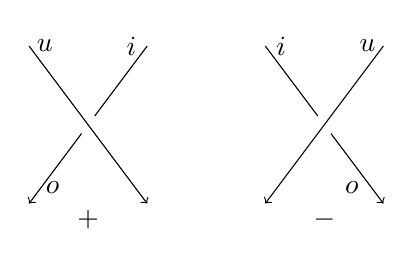
\begin{tikzpicture}
    \draw[<-] (0, -2)--(1.5, 0);
    \fill[white] (0.75, -1) circle (4pt);
    \draw[->] (0, 0)--(1.5, -2);

    \node at (0.75, -2.2) {$+$};
    \node at (0.2, 0) {$u$};
    \node at (1.3, 0) {$i$};
    \node at (0.3, -1.8) {$o$};

    \draw[->] (3, 0)--(4.5, -2);
    \fill[white] (3.75, -1) circle (4pt);
    \draw[<-] (3, -2)--(4.5, 0);
    
    \node at (3.75, -2.2) {$-$};
    \node at (3.2, 0) {$i$};
    \node at (4.3, 0) {$u$};
    \node at (4.1, -1.8) {$o$};
  \end{tikzpicture}
  \caption{\label{fig:3:two:types:crossings}Two types of crossings in oriented knot diagram.}
\end{figure}

Just as before, elements from $M^s$ that map to $0$ element in $M^x$ are responsible for coloring of diagram being examined. 
